\documentclass{article}
\usepackage{graphicx}
\usepackage{lipsum}
\usepackage[T2A]{fontenc}
\usepackage[utf8]{inputenc}

\graphicspath{ {./Results/} }

% \title{Quick Sort}
% \author{Dadmo}
% \date{\today}

\begin{document}
% \maketitle
\begin{titlepage}
    \begin{center}
    $\newline$
    \vspace{3.3cm}
    
    {\LARGE\textbf{Лабораторна робота №7\\"Quick Sort"}}
    \vspace{10cm}
    \begin{flushright}
        \textbf{Роботу виконав:}\\Климентьєв Максим \\3-го курсу\\групи ФІ-21
    \end{flushright}
    \end{center}
\end{titlepage}
\newpage

\tableofcontents 
\section{Quick Sort}
\textbf{QuickSort} --- клас, який має реалiзованi 4 (16) варiантів алгоритму сортування.
\newline

\textbf{Реалiзовано 4 варiанти розбиття}: 
\begin{enumerate}
    \item Розбиття Ломуто
    \item Розбиття Гоара
    \item Розбиття Дейкстри
    \item Двоелементне Розбиття
\end{enumerate}

\textbf{Для кожно розбиття реалiзовано 4 варiанти вибору опорного елемента}:
\begin{enumerate}
    \item Останній елемент
    \item Випадковий елемент
    \item Медіана першого, середнього та останього елемента
    \item Медіана трьох випадкових елементів
\end{enumerate}

Маю трохи не таку, як на лекції, реалізацію для розбиття Гоара та двохстороньового розбиття, оскільки опорні елементи вилучаю, а в кінці додаю на необхідне місце.
\newline
\indent Через це розбиття Гоара робить більше порівнянь, але менше операцій обміну.
\newline

\section{Quick Sort Test}
\textbf{Перевіряє чи масив відсортований завдяки певній варіації алгоритму чи ні.}

\section{Random Lists}
\textbf{RandomLists} --- клас, який має реалiзованi 6 варiантів генерацiї спискiв.
\begin{enumerate}
    \item \textbf{Повнiстю вiдсортований (sorted)} --- на вхід подається лише розмiр списку.
    \item \textbf{Випадковi (random)} --- на вхід подається лише розмiр списку.
    \item \textbf{Майже вiдсортований (almostsorted)} --- на вхід подається розмiр списку, та відсоток безпорядку.
    \item \textbf{Вiдсортованi в зворотному порядку (reverse)} --- на вхід подається лише розмiр списку.
    \item \textbf{Лише з декiлькома рiзними значеннями (somenumbers)} --- на вхід подається розмiр списку, та діапазон значень (Початок, Кiнець).
    \item \textbf{"Трикутнi" (triangular)} (перша половина є строго висхiдною послiдовнiстю, а друга половина є дзеркальним вiдображенням першої).
\end{enumerate}
\newpage

\section{Comparisions and Results}
% SORTED
    \subsection{Результати для відсортованих масивів:}
    \textbf{Час виконання:}
    \newline
        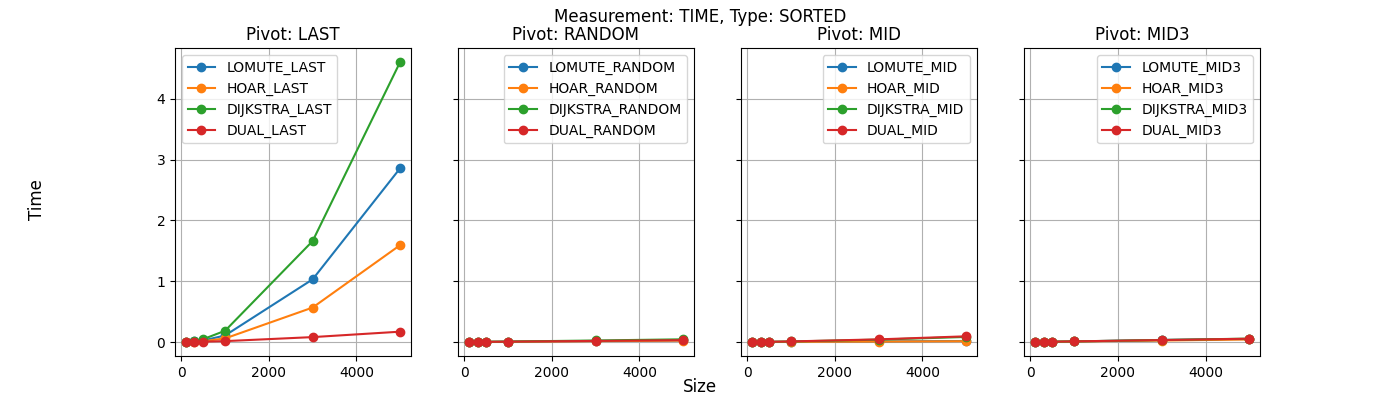
\includegraphics[scale=0.5]{sorted_Time_6_numbers.png}
        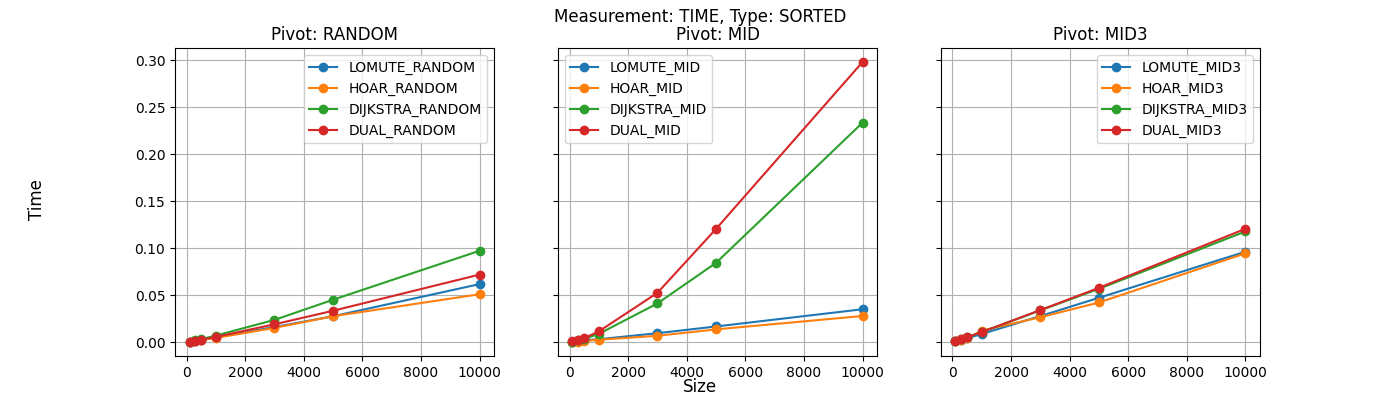
\includegraphics[scale=0.5]{sorted_Time_3_pivots_7_numbers.png}
    \textbf{Кiлькiсть проведених порiвнянь:}
    \newline
        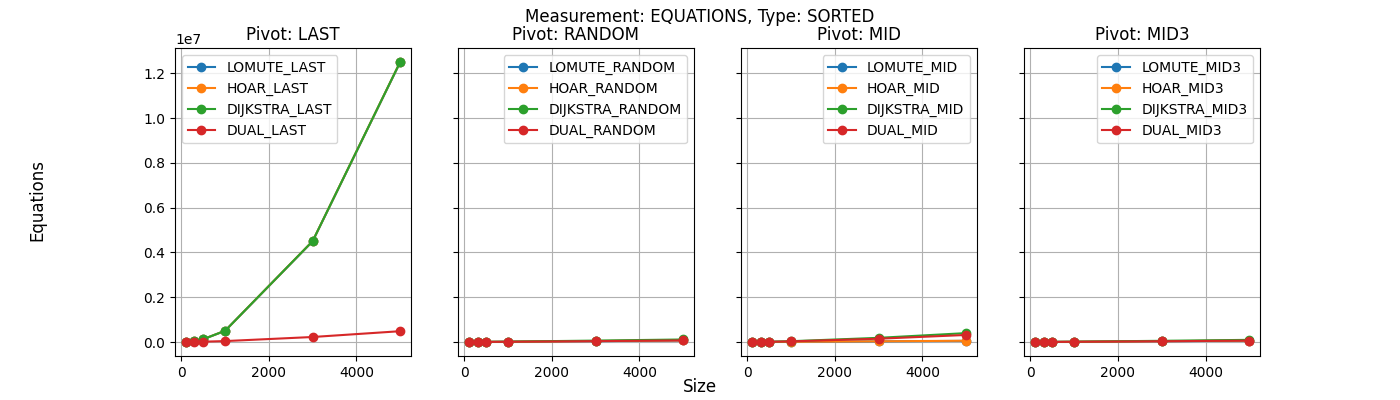
\includegraphics[scale=0.5]{sorted_Equations_6_numbers.png}
        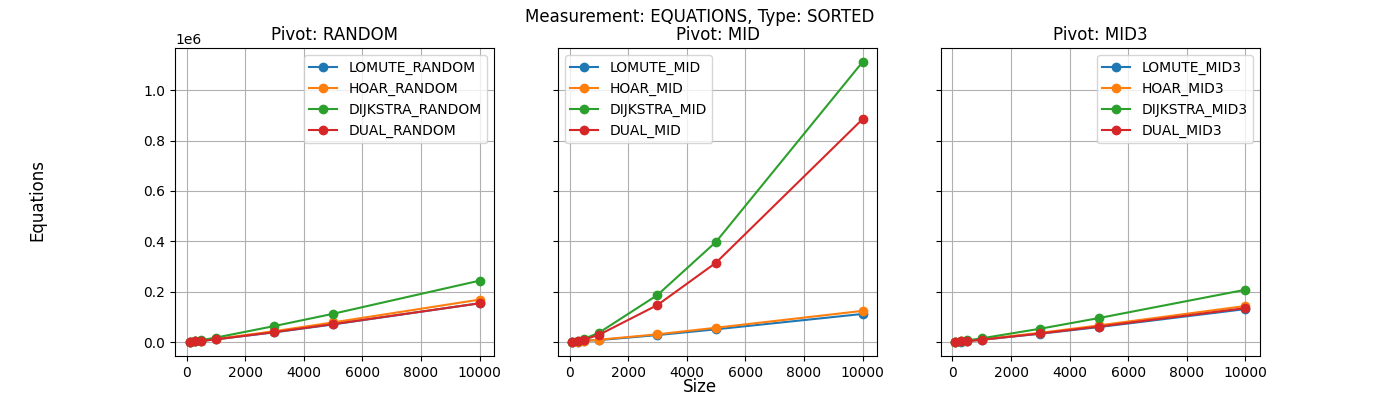
\includegraphics[scale=0.5]{sorted_Equations_3_pivots_7_numbers.png}
        \newline
    \textbf{Операцiй обмінів:}
    \newline
        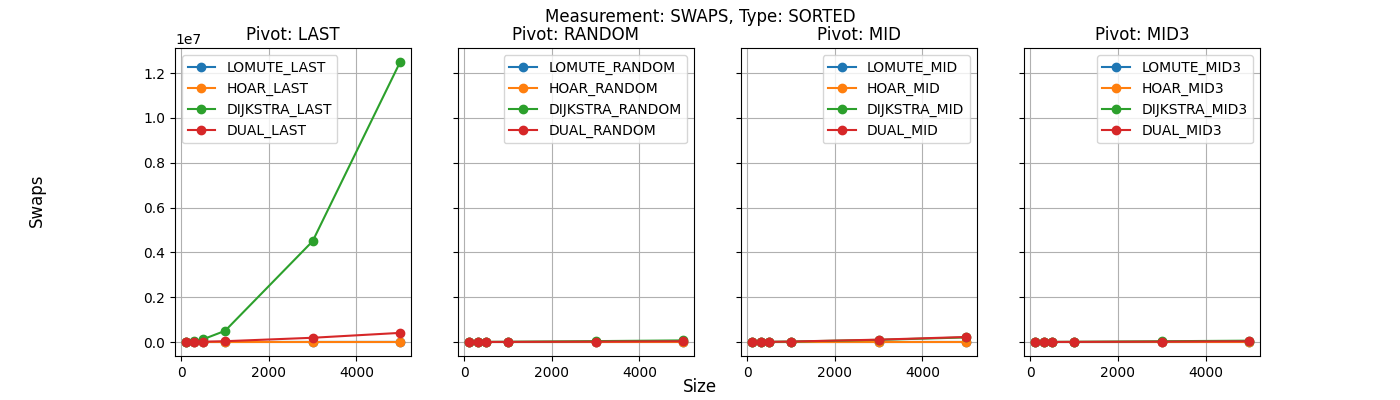
\includegraphics[scale=0.5]{sorted_Swaps_6_numbers.png}
        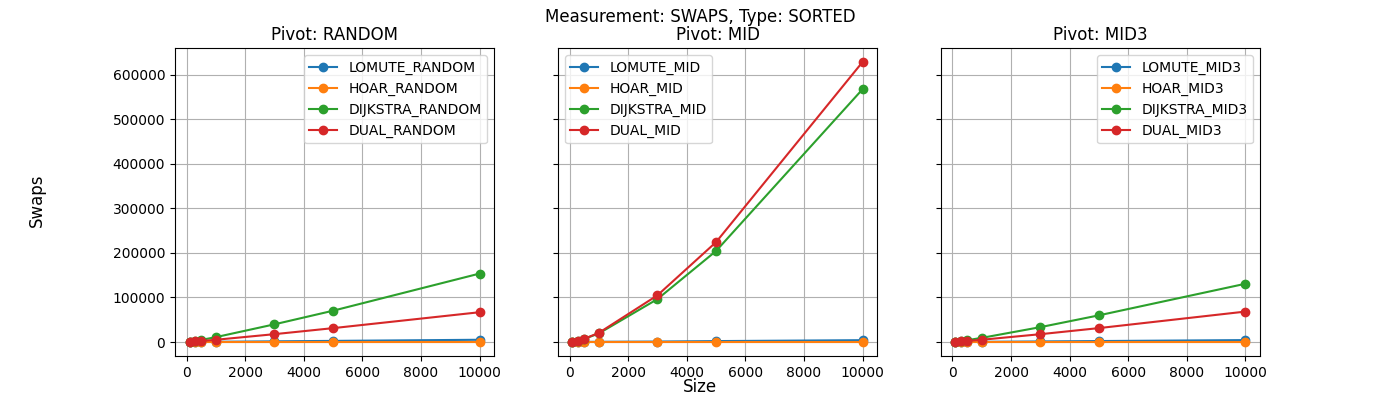
\includegraphics[scale=0.5]{sorted_Swaps_3_pivots_7_numbers.png}
        \newline
    \newpage
    \textbf{Використано пам’ятi:}
    \newline
        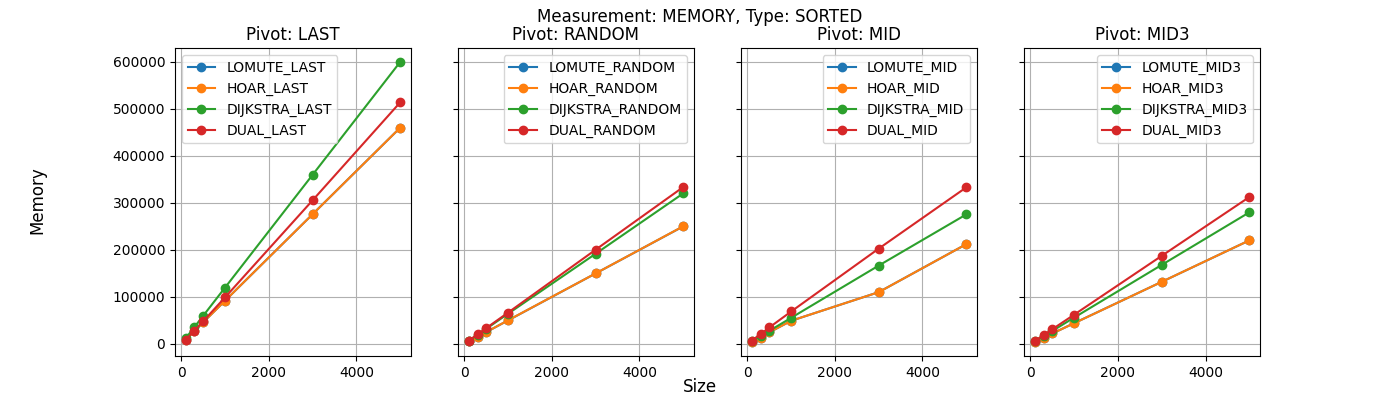
\includegraphics[scale=0.5]{sorted_Memory_6_numbers.png}
        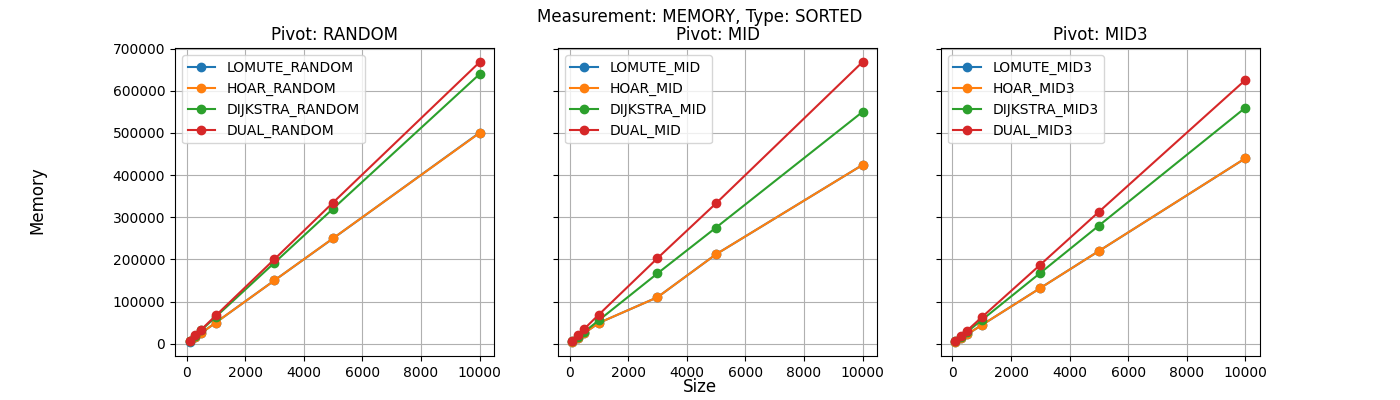
\includegraphics[scale=0.5]{sorted_Memory_3_pivots_7_numbers.png}
    \subsection{Висновки для відсортованих масивів:}
    \begin{enumerate}
        \item Усі розбиття дуже довго рахують коли опорний елемент обирається як останній.
        \item Розбиття Дейкстри дуже багато порівнянь та обмінів використовує коли опорний елемент обирається як останній.
        \item Найбільше пам'яті використовується коли обирається останній елемент як опорний.
    \end{enumerate}
    \newpage

% RANDOM
    \subsection{Результати для масивів випадкових елементів:}
    \textbf{Час виконання:}
    \newline
        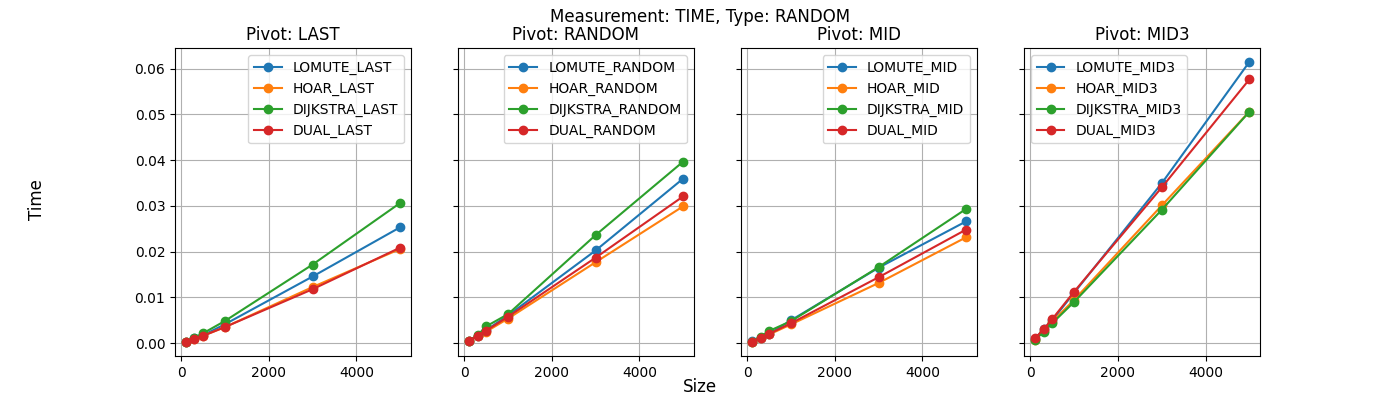
\includegraphics[scale=0.5]{random_Time_6_numbers.png}
        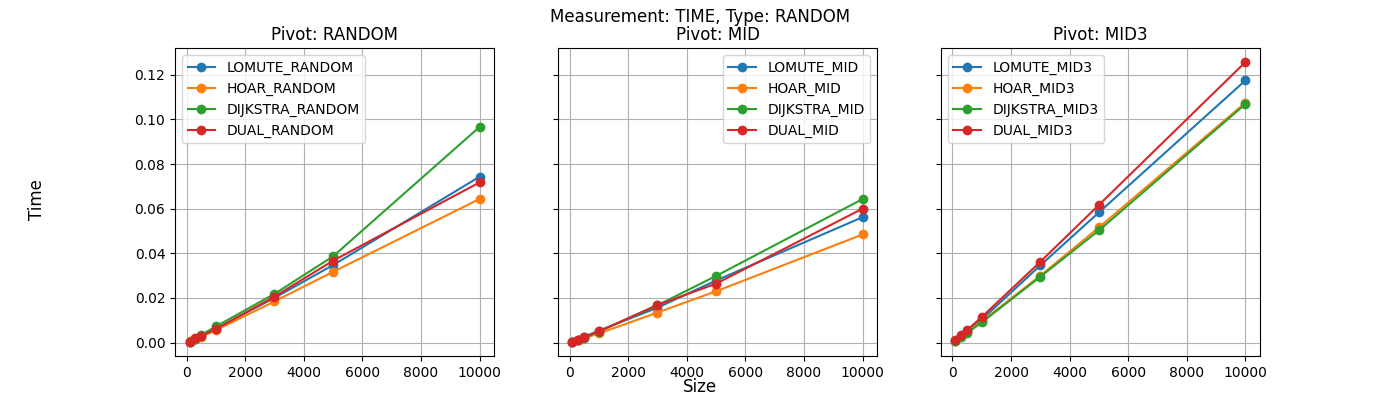
\includegraphics[scale=0.5]{random_Time_3_pivots_7_numbers.png}
    \textbf{Кiлькiсть проведених порiвнянь:}
    \newline
        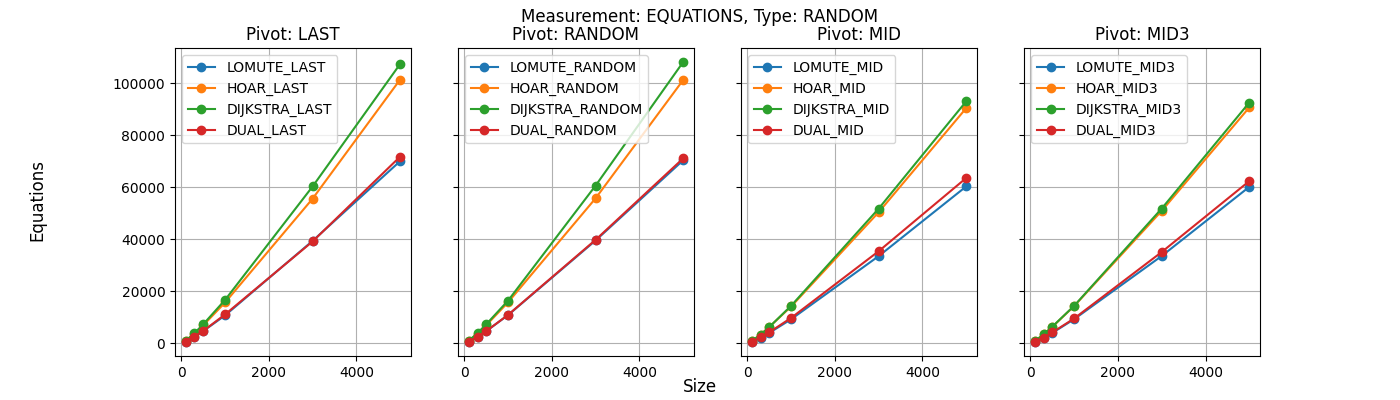
\includegraphics[scale=0.5]{random_Equations_6_numbers.png}
        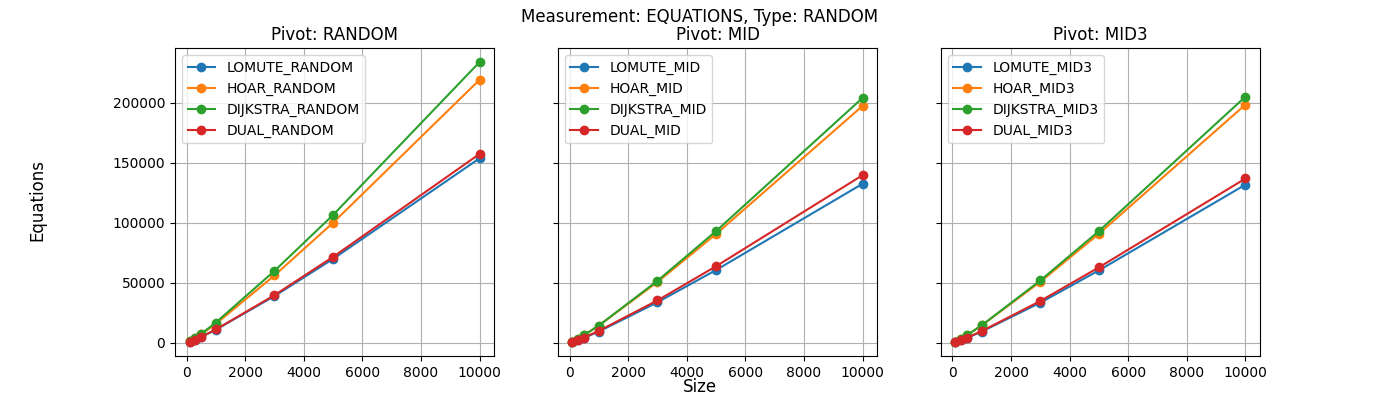
\includegraphics[scale=0.5]{random_Equations_3_pivots_7_numbers.png}
        \newline
    \textbf{Операцiй обмінів:}
    \newline
        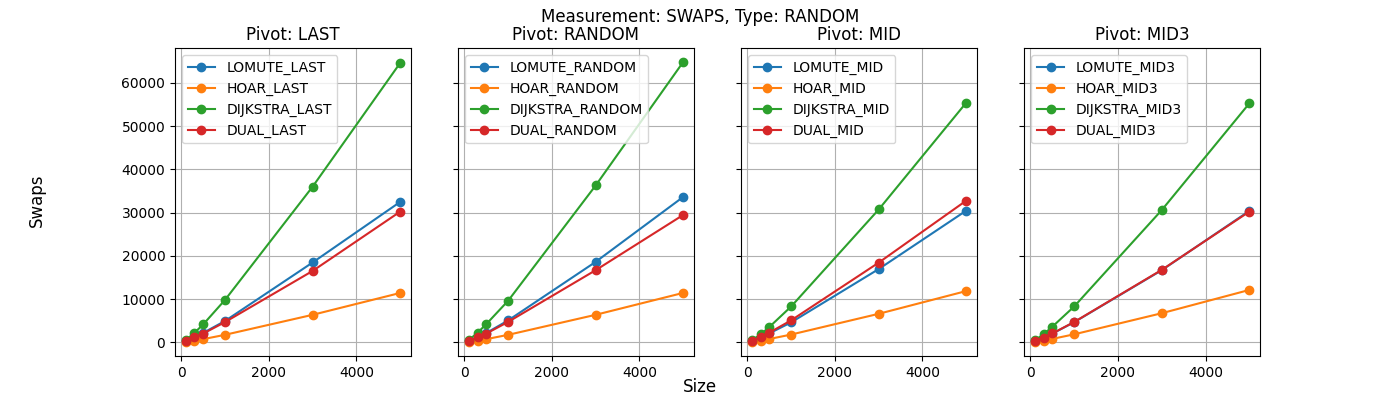
\includegraphics[scale=0.5]{random_Swaps_6_numbers.png}
        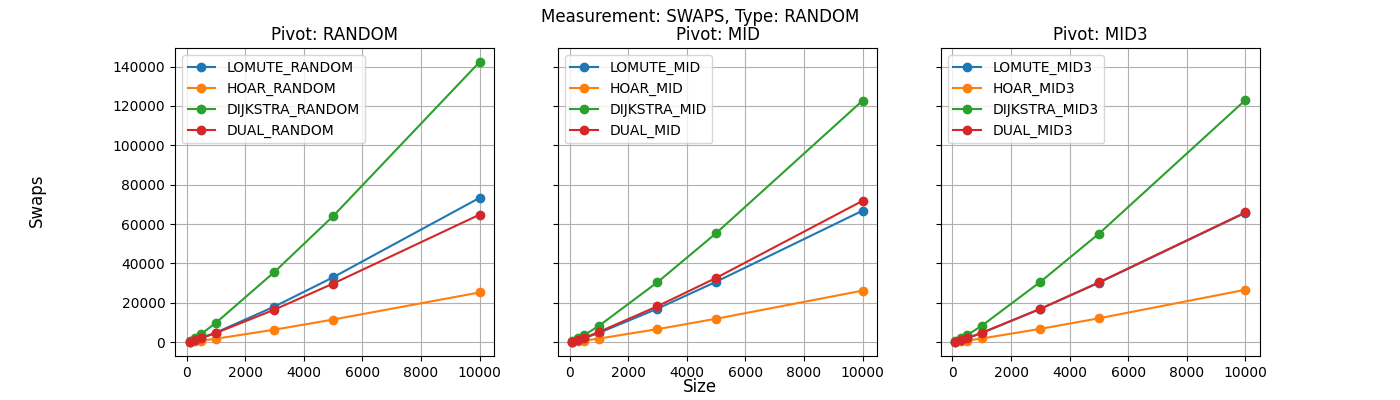
\includegraphics[scale=0.5]{random_Swaps_3_pivots_7_numbers.png}
        \newline
    \newpage
    \textbf{Використано пам’ятi:}
    \newline
        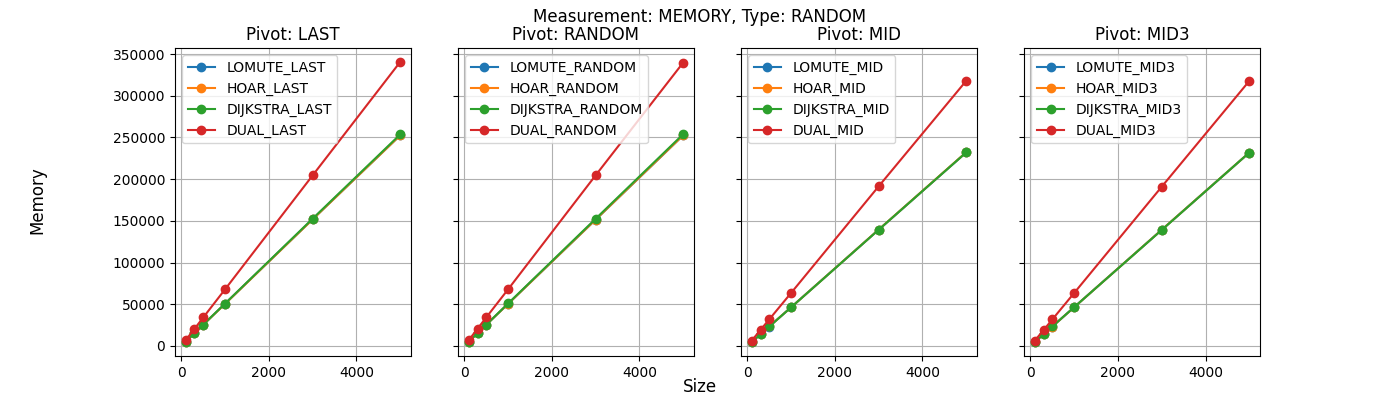
\includegraphics[scale=0.5]{random_Memory_6_numbers.png}
        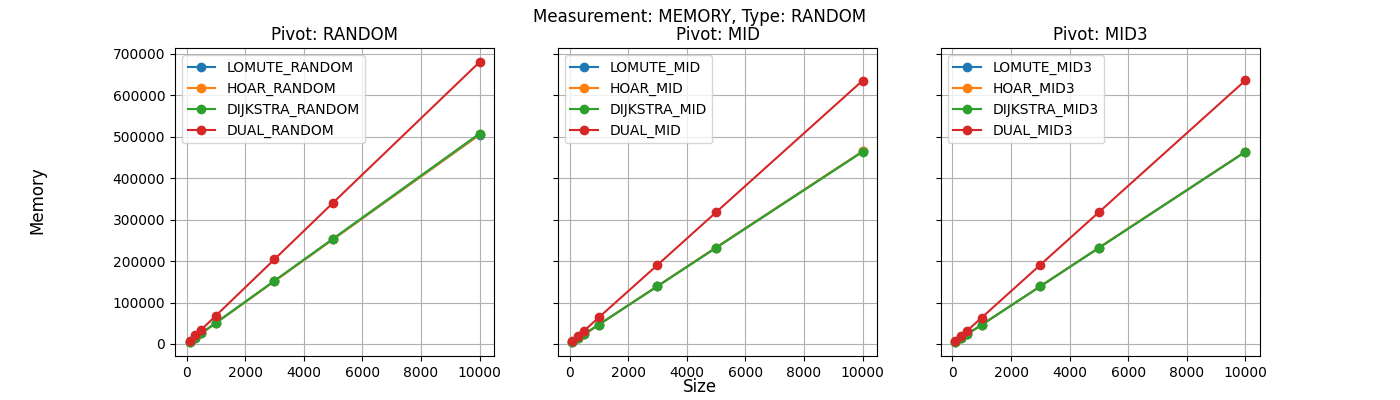
\includegraphics[scale=0.5]{random_Memory_3_pivots_7_numbers.png}
    \subsection{Висновки для масивів випадкових елементів:}
    \begin{enumerate}
        \item Для масивів з випадковими елементами обрання опорного елемента як медіани трьох випадкових елементів дуже багато часу використовує.
        \item обрання опорного елементу як медіани першого, середнього та останього елемента використовує порівняно з іншим менше порівнянь, обмінів та пам'ятi.
        \item Дейкстра вийшла майже завжди найгірша по часу, кількості порівнянь та обмінів, але краща по пам'яті.
    \end{enumerate}
    \newpage

% ALMOST SORTED
    \subsection{Результати для майже відсортованих масивів:}
    \textbf{Час виконання:}
    \newline
        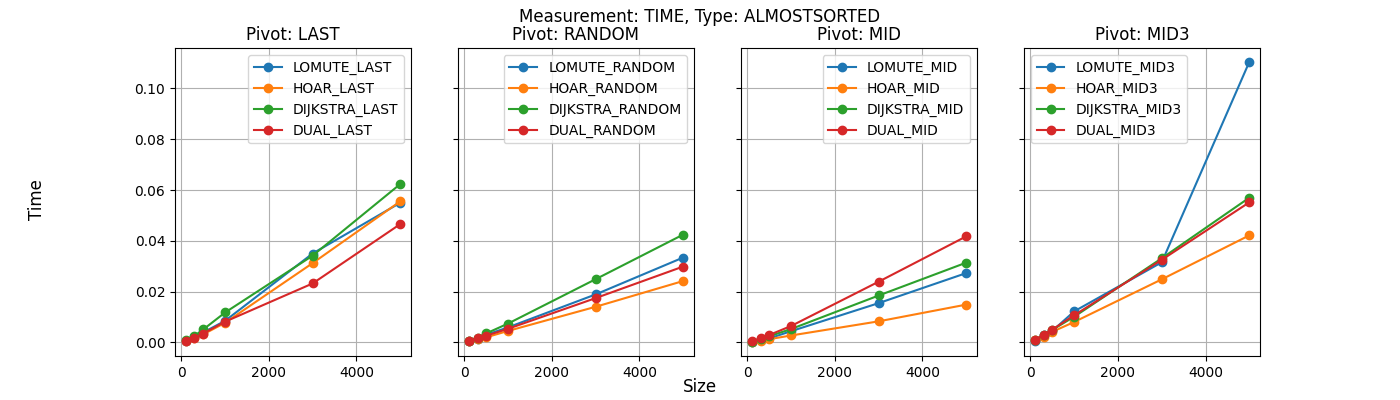
\includegraphics[scale=0.5]{almostsorted_Time_6_numbers.png}
        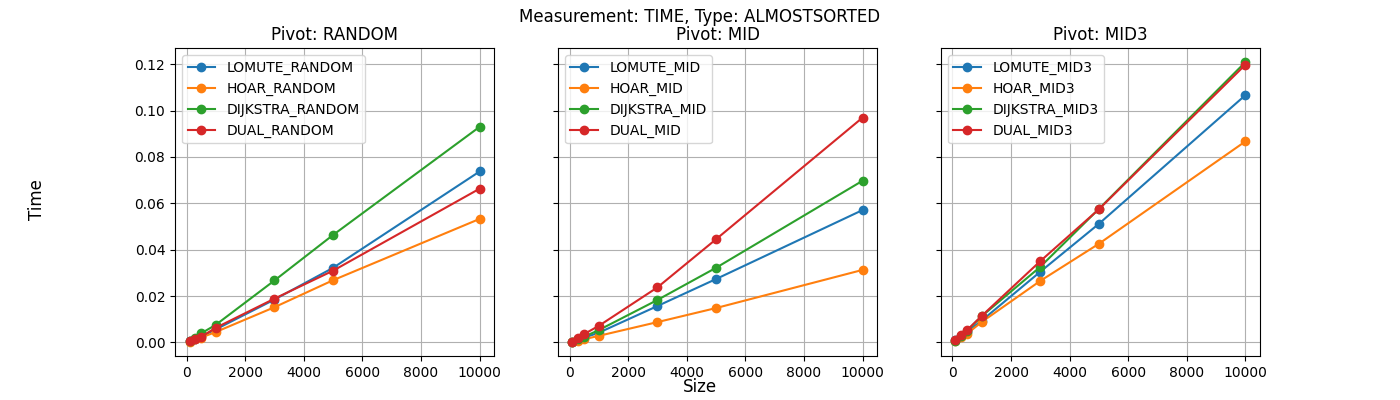
\includegraphics[scale=0.5]{almostsorted_Time_3_pivots_7_numbers.png}
    \textbf{Кiлькiсть проведених порiвнянь:}
    \newline
        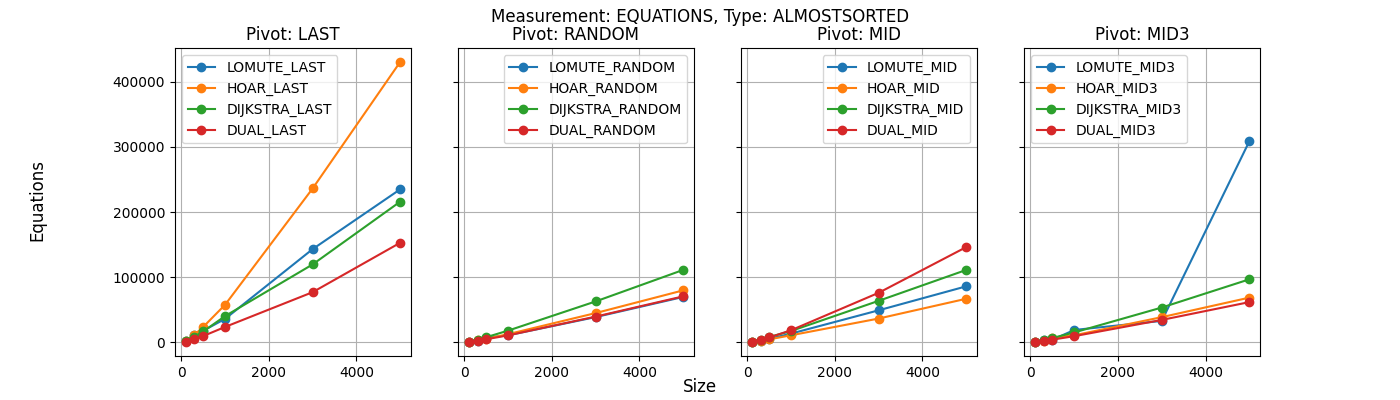
\includegraphics[scale=0.5]{almostsorted_Equations_6_numbers.png}
        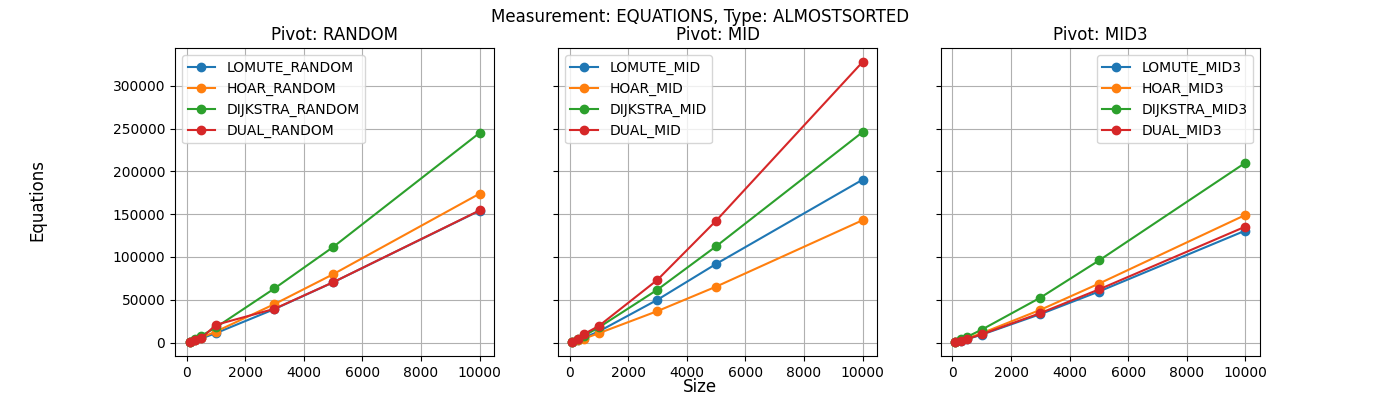
\includegraphics[scale=0.5]{almostsorted_Equations_3_pivots_7_numbers.png}
        \newline
    \textbf{Операцiй обмінів:}
    \newline
        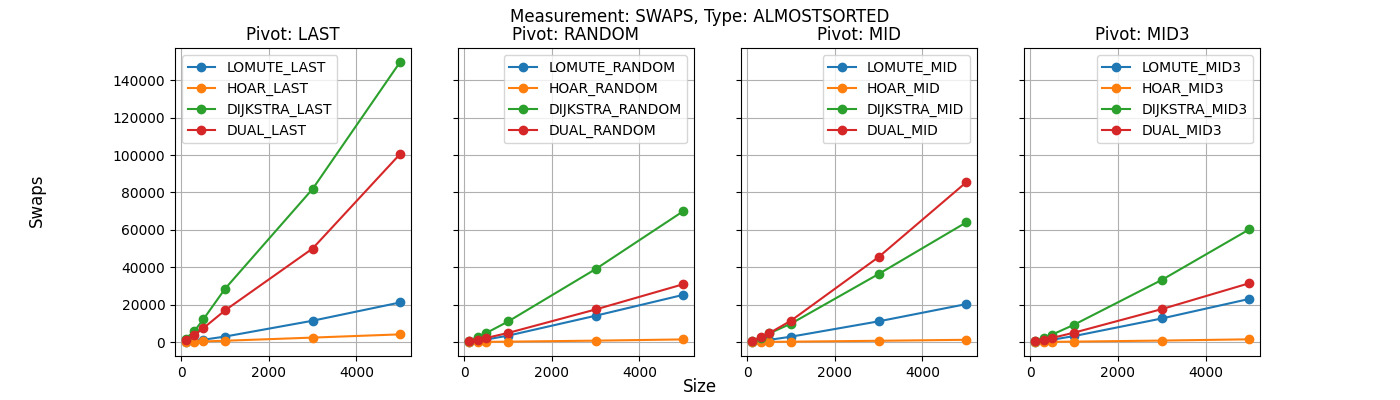
\includegraphics[scale=0.5]{almostsorted_Swaps_6_numbers.png}
        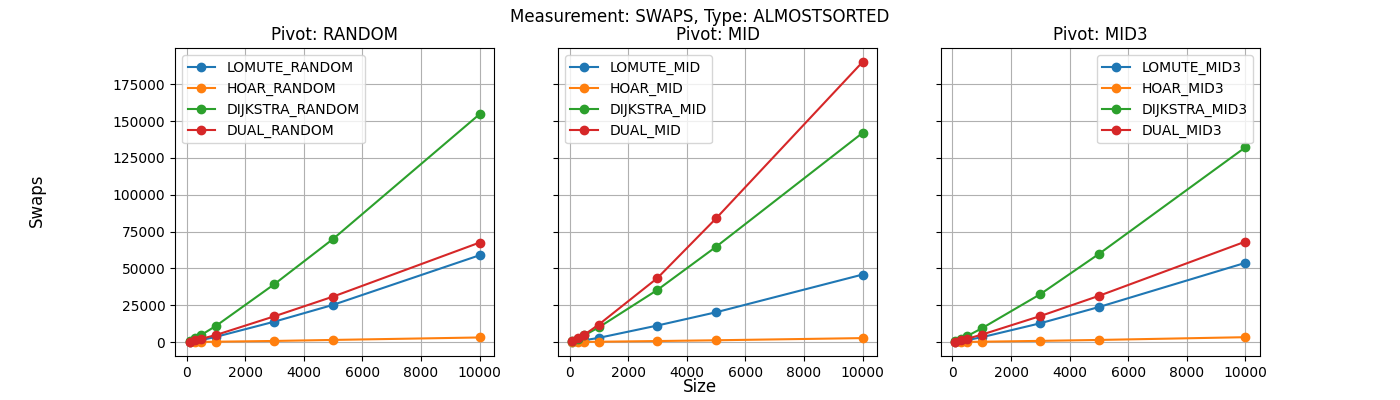
\includegraphics[scale=0.5]{almostsorted_Swaps_3_pivots_7_numbers.png}
        \newline
    \newpage
    \textbf{Використано пам’ятi:}
    \newline
        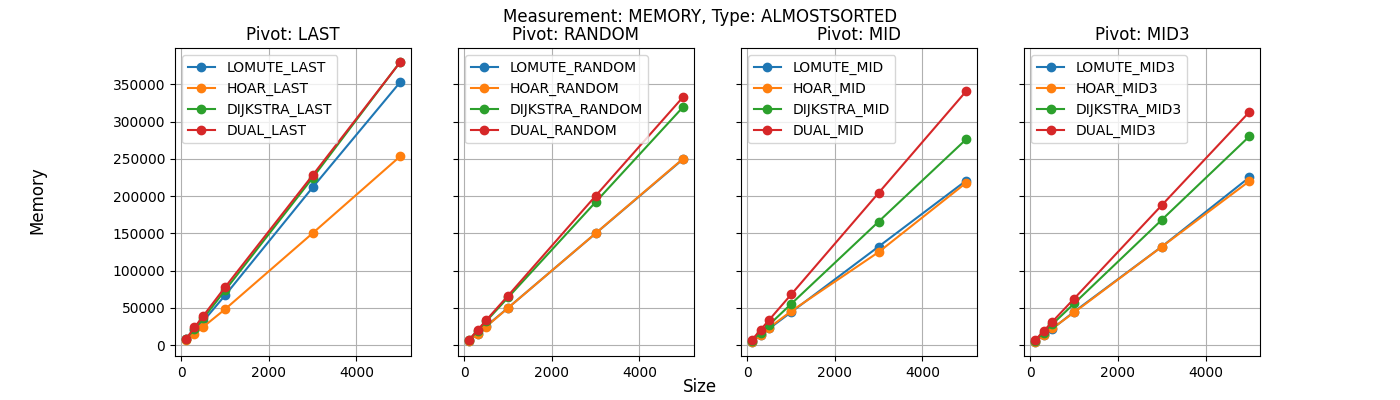
\includegraphics[scale=0.5]{almostsorted_Memory_6_numbers.png}
        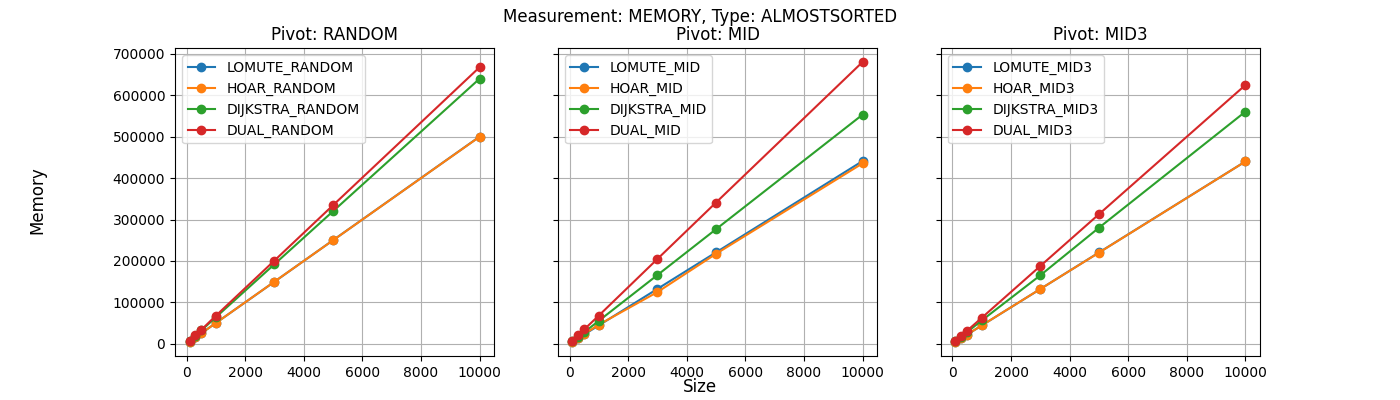
\includegraphics[scale=0.5]{almostsorted_Memory_3_pivots_7_numbers.png}
    \subsection{Висновки для майже відсортованих масивів:}
    \begin{enumerate}
        \item Для майже відсортованих масивів обрання опорного елемента як медіани трьох випадкових елементів багато часу використовує, особливо для розбиття Ломуто.
        \item Гоар робить багато порівнянь, коли опорний елемент обирається як останній, а Ломуто коли як медіана трьох випадкових елементів.
        \item Дейкстра робить багата обмінів, коли опорний елементи обирається як останній.
    \end{enumerate}
    \newpage

% REVERSE
    \subsection{Результати для відсортованих у зворотному напрямку масивів:}
    \textbf{Час виконання:}
    \newline
        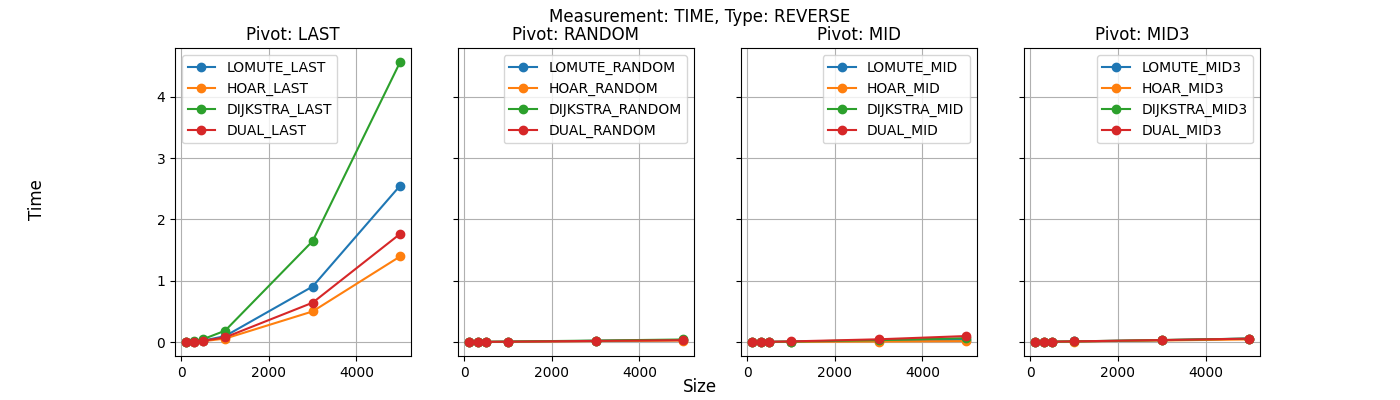
\includegraphics[scale=0.5]{reverse_Time_6_numbers.png}
        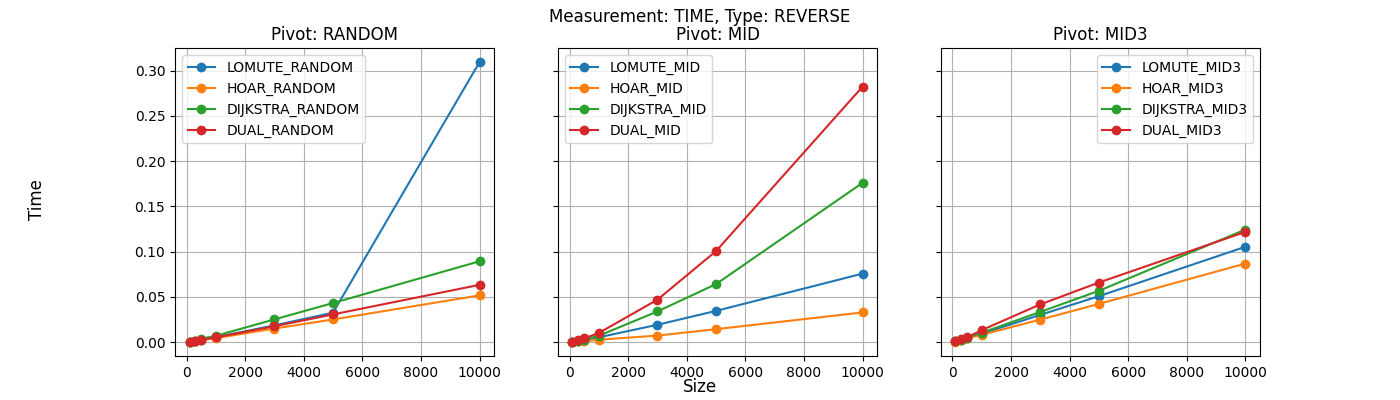
\includegraphics[scale=0.5]{reverse_Time_3_pivots_7_numbers.png}
    \textbf{Кiлькiсть проведених порiвнянь:}
    \newline
        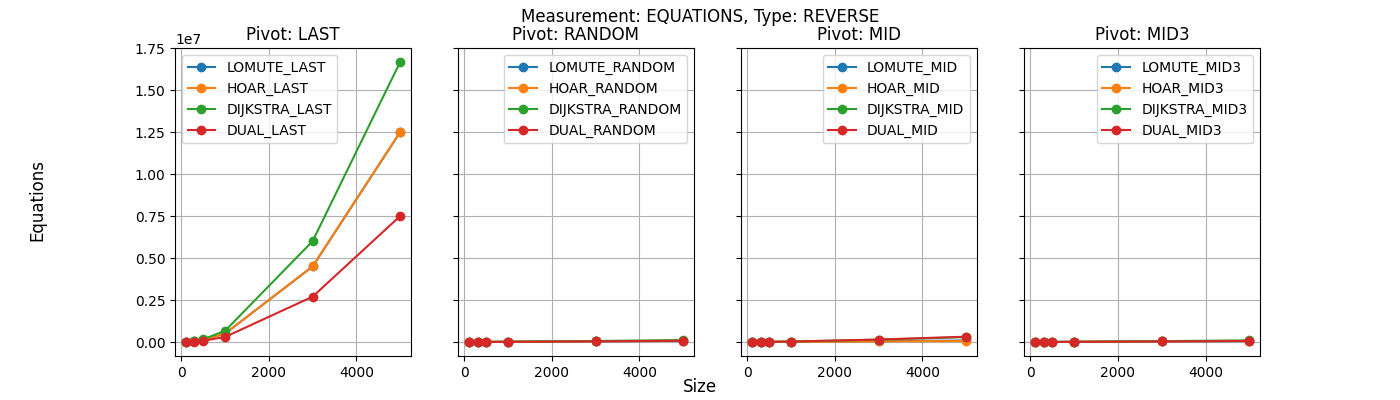
\includegraphics[scale=0.5]{reverse_Equations_6_numbers.png}
        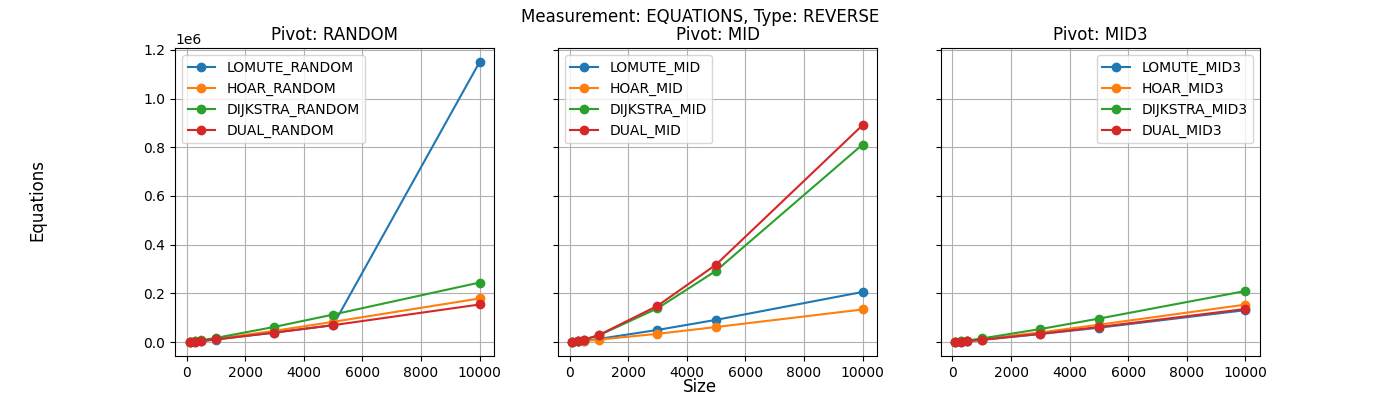
\includegraphics[scale=0.5]{reverse_Equations_3_pivots_7_numbers.png}
        \newline
    \textbf{Операцiй обмінів:}
    \newline
        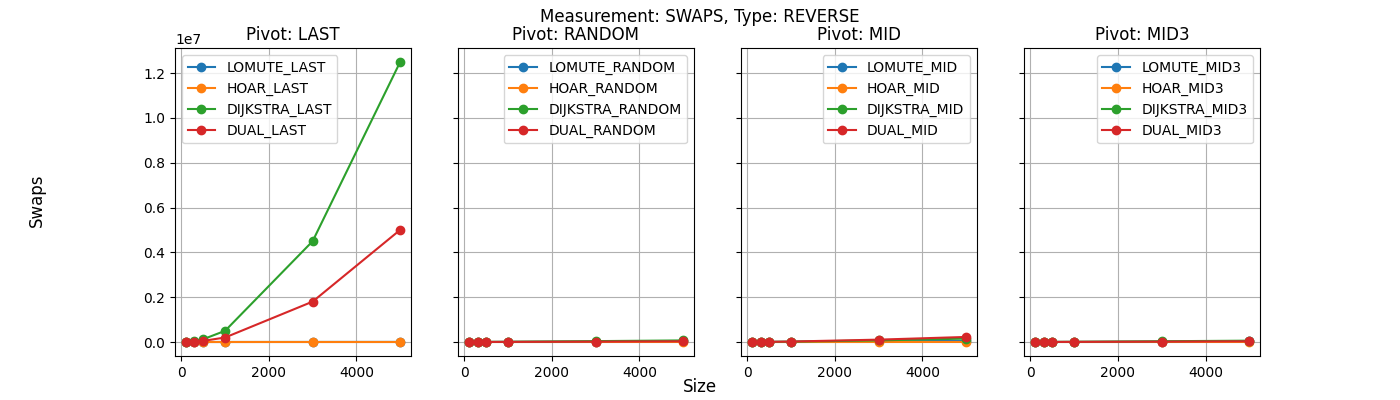
\includegraphics[scale=0.5]{reverse_Swaps_6_numbers.png}
        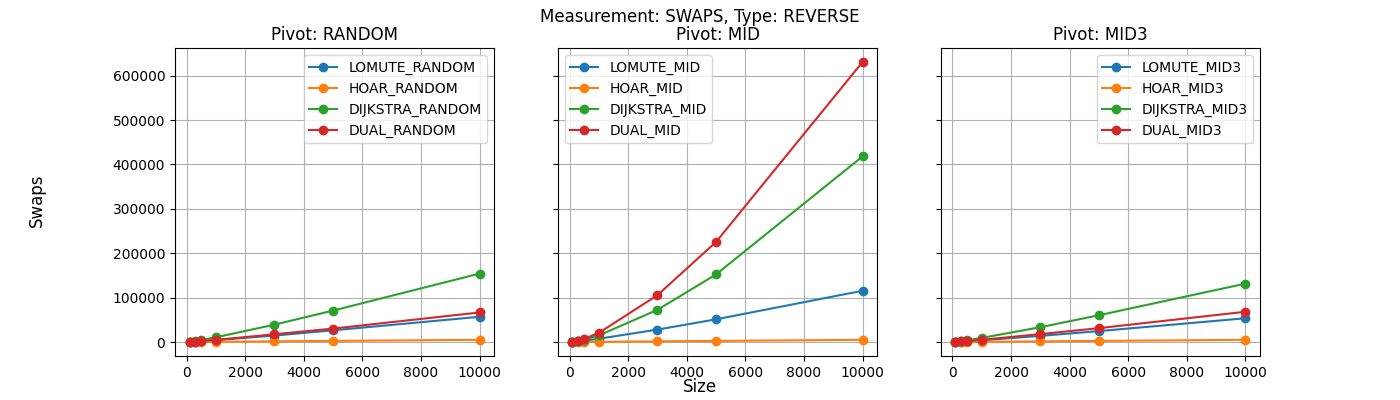
\includegraphics[scale=0.5]{reverse_Swaps_3_pivots_7_numbers.png}
        \newline
    \newpage
    \textbf{Використано пам’ятi:}
    \newline
        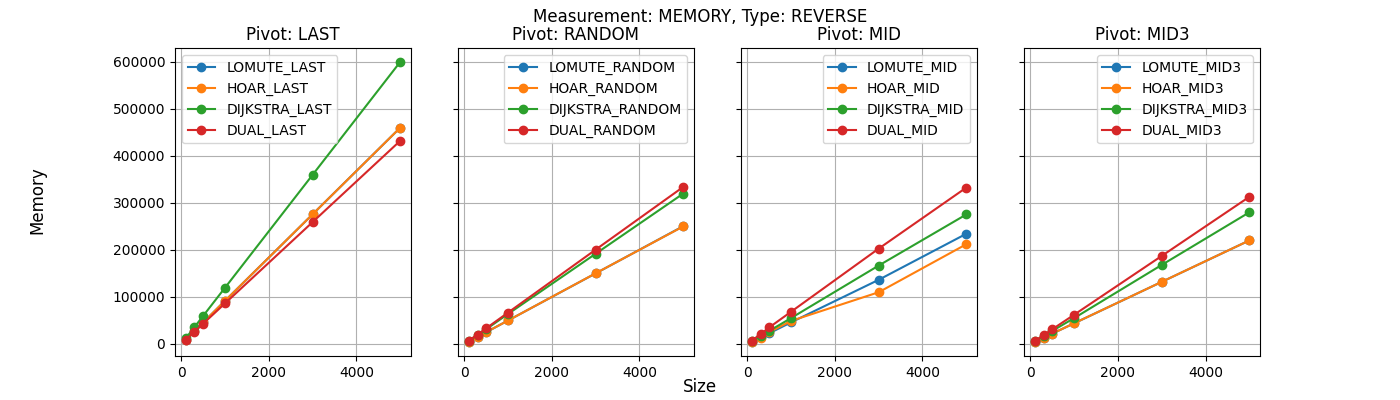
\includegraphics[scale=0.5]{reverse_Memory_6_numbers.png}
        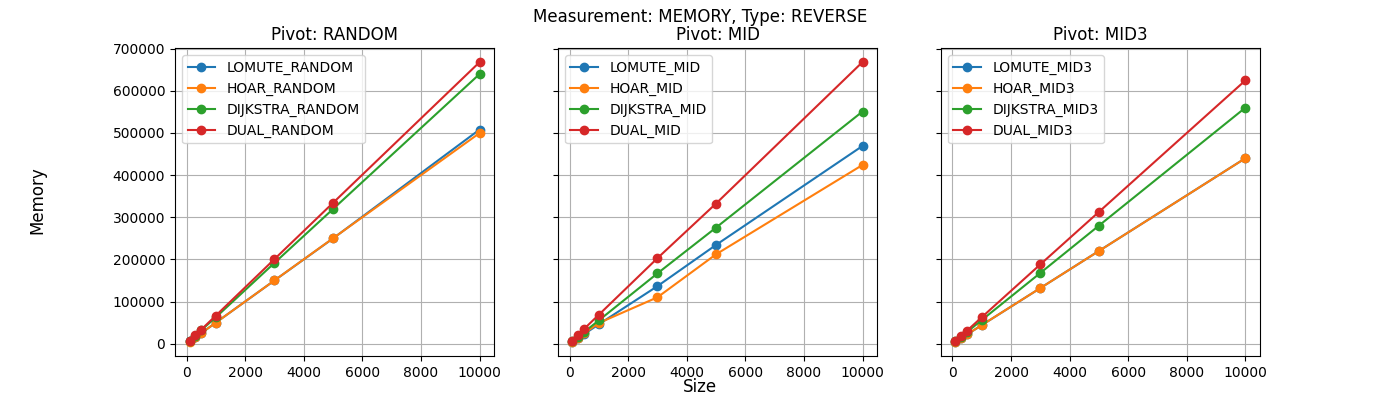
\includegraphics[scale=0.5]{reverse_Memory_3_pivots_7_numbers.png}
    \subsection{Висновки для відсортованих у зворотному напрямку масивів:}
    \begin{enumerate}
        \item Дуже багато часу займає, коли опорний елемент обирається як останній, через те, що два масиви, що він отримує є дуже не збалансованими по розміру, один масив має на один елемент менше, а другий не має елементів взагалі.
        \item 
    \end{enumerate}
    \newpage

%  SOMENUMBERS
    \subsection{Результати для масивів лише з декількома значеннями:}
    \textbf{Час виконання:}
    \newline
        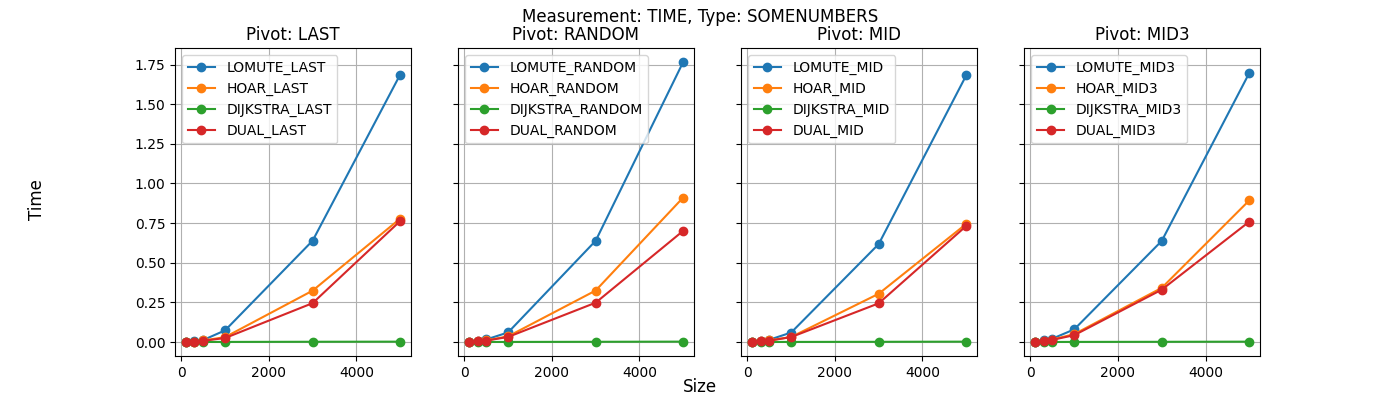
\includegraphics[scale=0.5]{somenumbers_Time_6_numbers.png}
        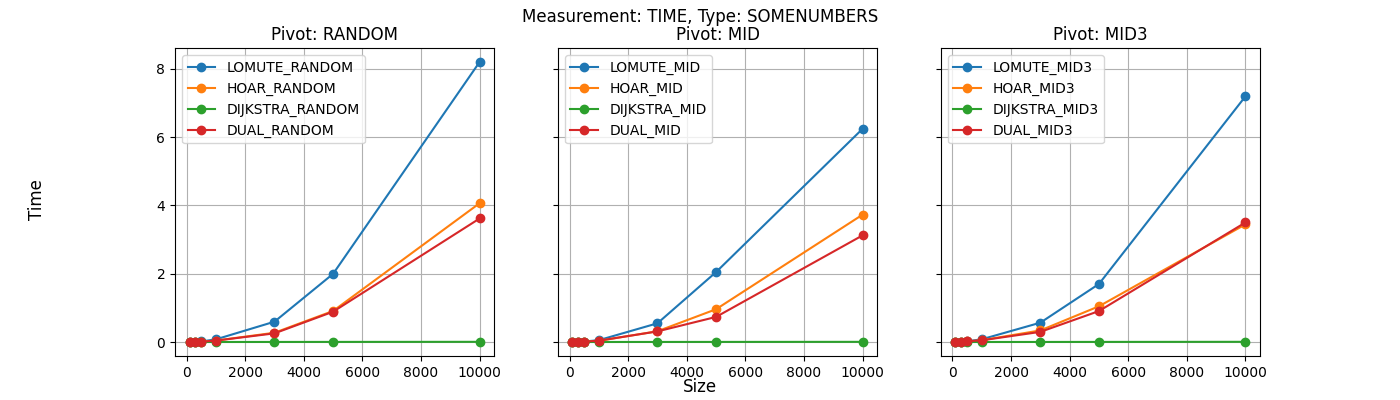
\includegraphics[scale=0.5]{somenumbers_Time_3_pivots_7_numbers.png}
    \textbf{Кiлькiсть проведених порiвнянь:}
    \newline
        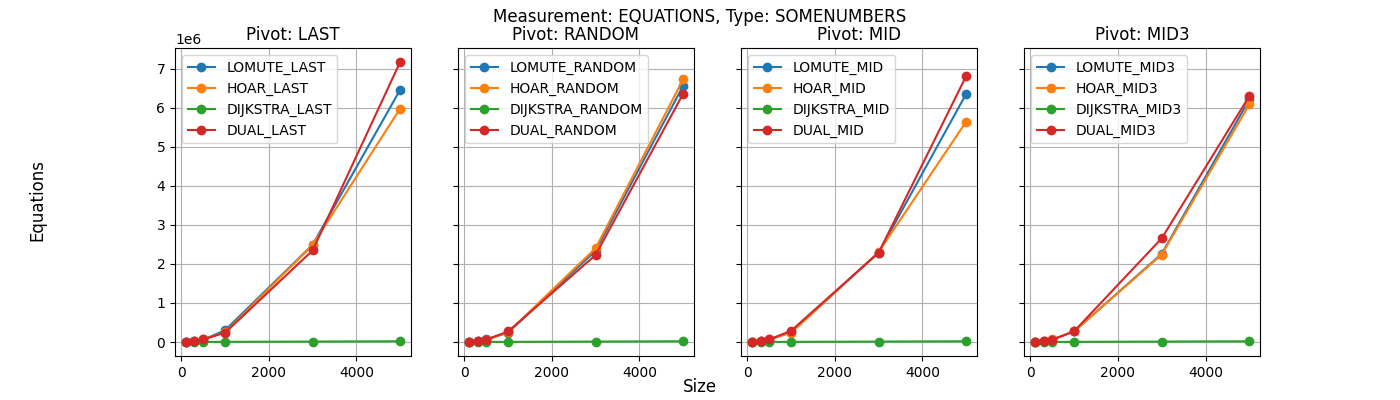
\includegraphics[scale=0.5]{somenumbers_Equations_6_numbers.png}
        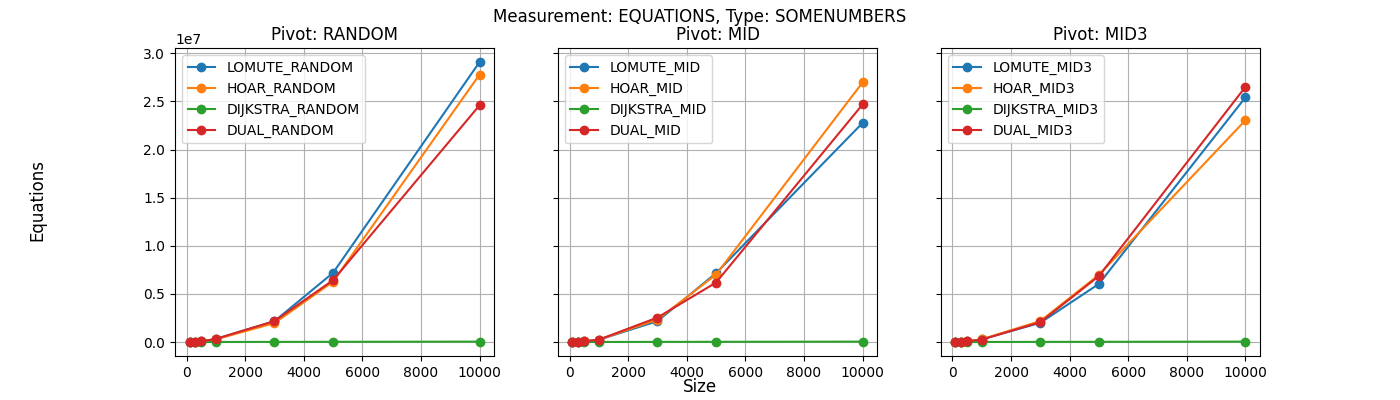
\includegraphics[scale=0.5]{somenumbers_Equations_3_pivots_7_numbers.png}
        \newline
    \textbf{Операцiй обмінів:}
    \newline
        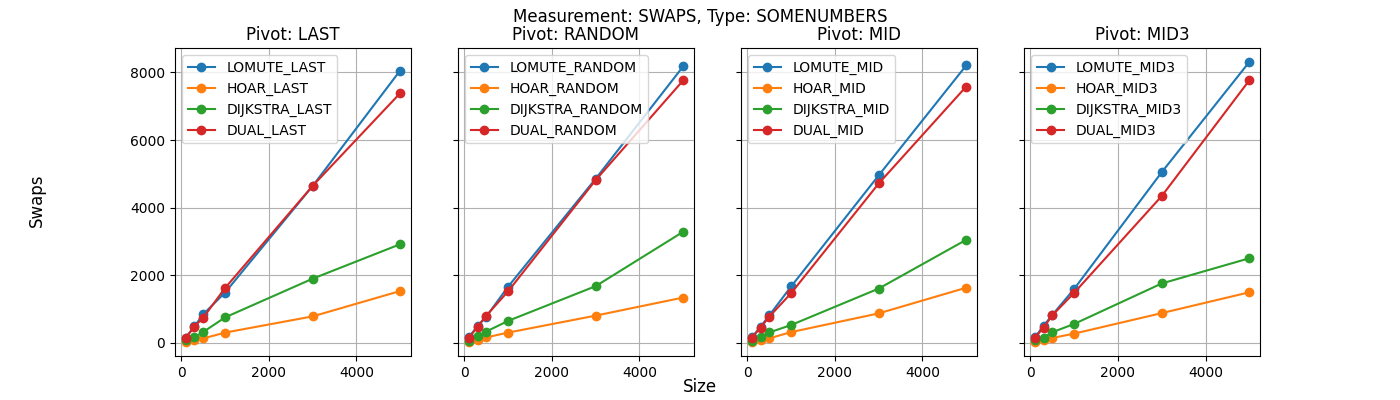
\includegraphics[scale=0.5]{somenumbers_Swaps_6_numbers.png}
        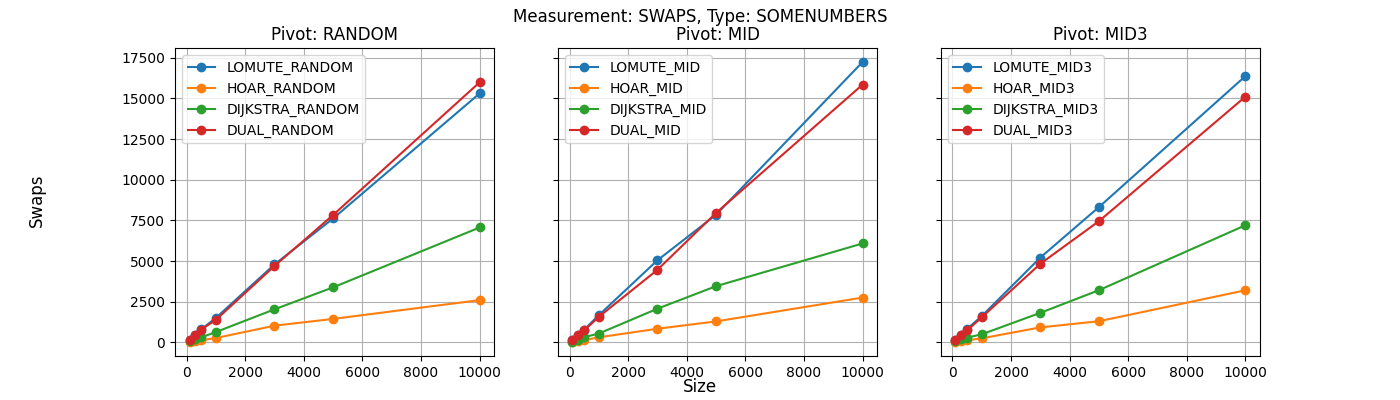
\includegraphics[scale=0.5]{somenumbers_Swaps_3_pivots_7_numbers.png}
        \newline
    \newpage
    \textbf{Використано пам’ятi:}
    \newline
        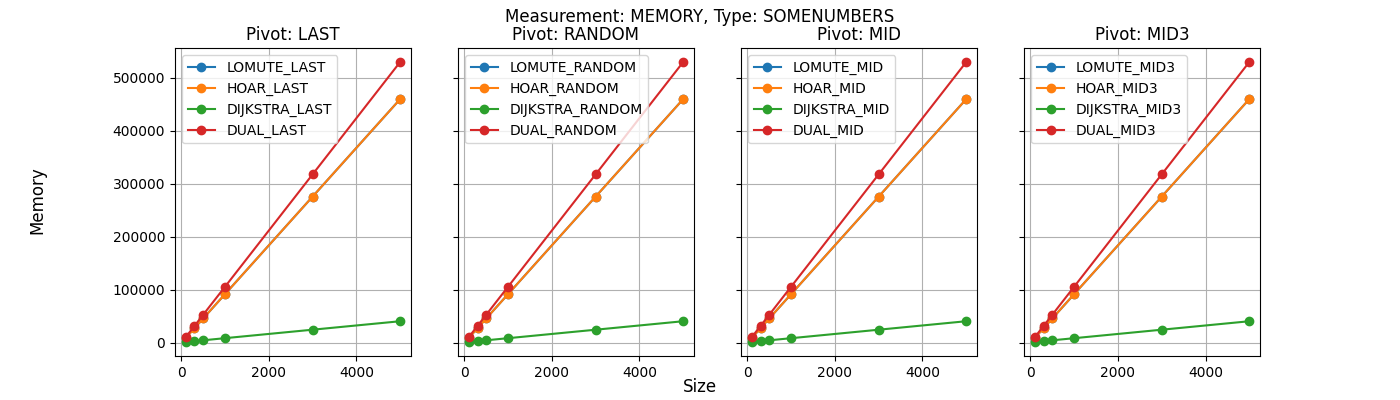
\includegraphics[scale=0.5]{somenumbers_Memory_6_numbers.png}
        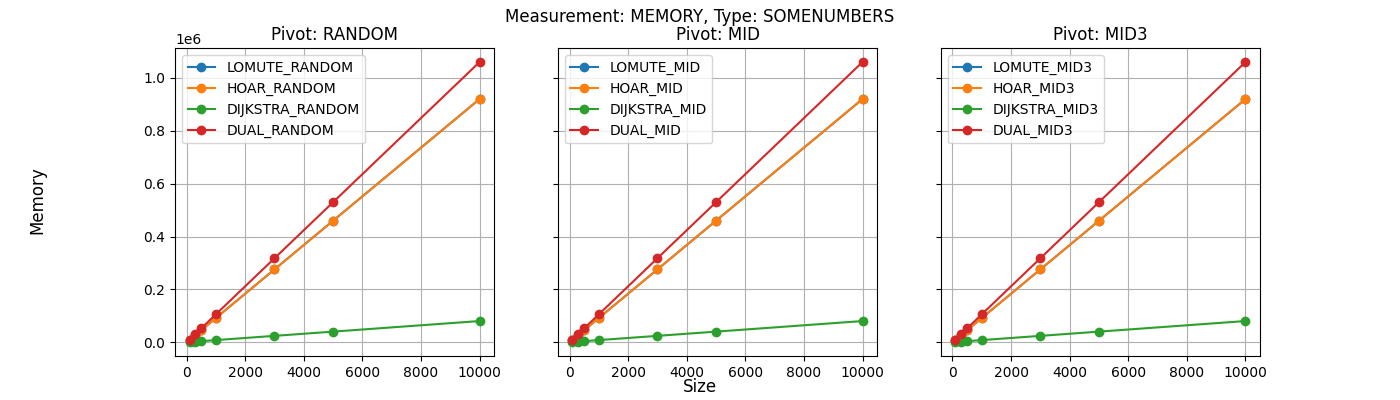
\includegraphics[scale=0.5]{somenumbers_Memory_3_pivots_7_numbers.png}
    \subsection{Висновки для масивів лише з декількома значеннями:}
    \begin{enumerate}
        \item 
    \end{enumerate}
    \newpage

% TRIANGULAR
    \subsection{Результати для "трикутних" масивів:}
    \textbf{Час виконання:}
    \newline
        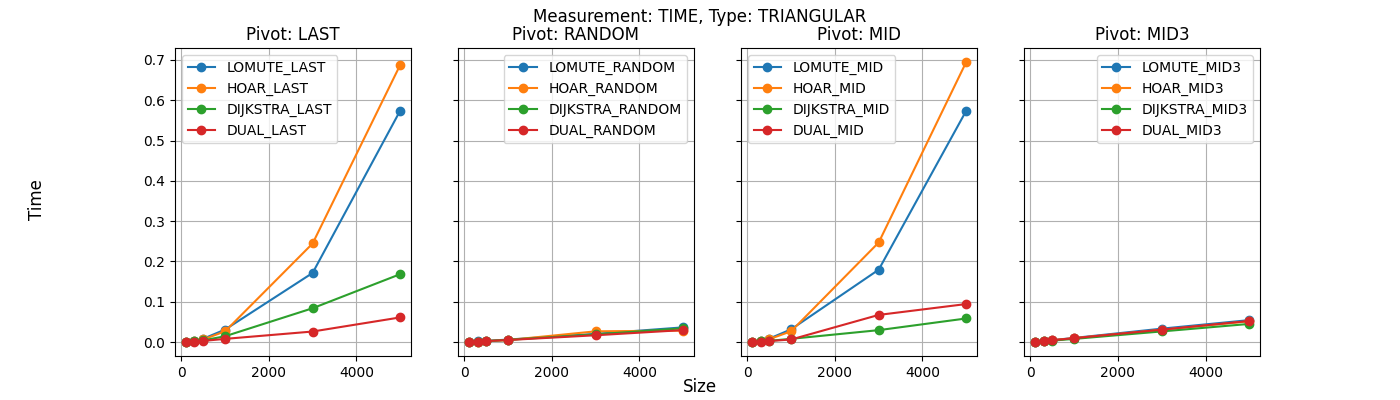
\includegraphics[scale=0.5]{triangular_Time_6_numbers.png}
        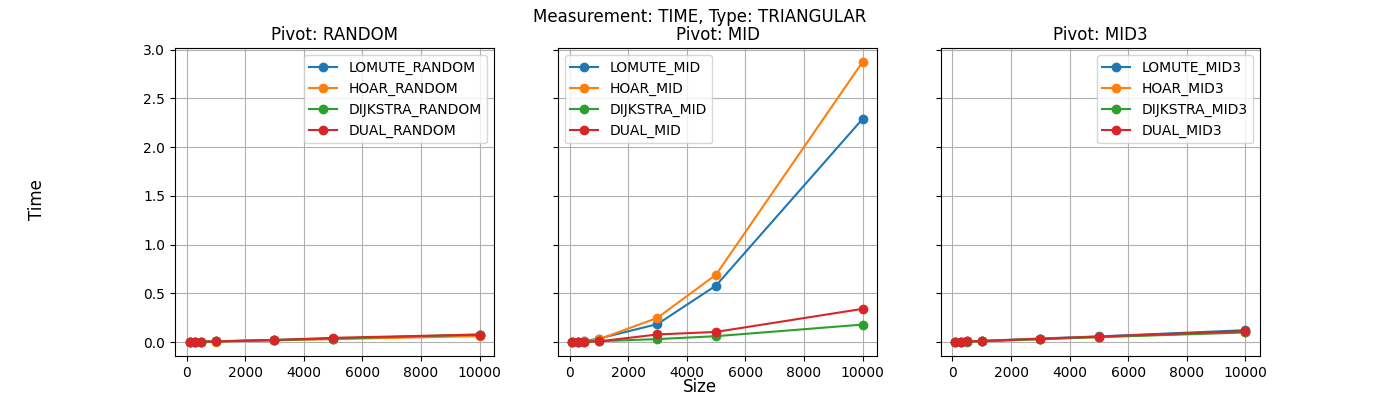
\includegraphics[scale=0.5]{triangular_Time_3_pivots_7_numbers.png}
    \textbf{Кiлькiсть проведених порiвнянь:}
    \newline
        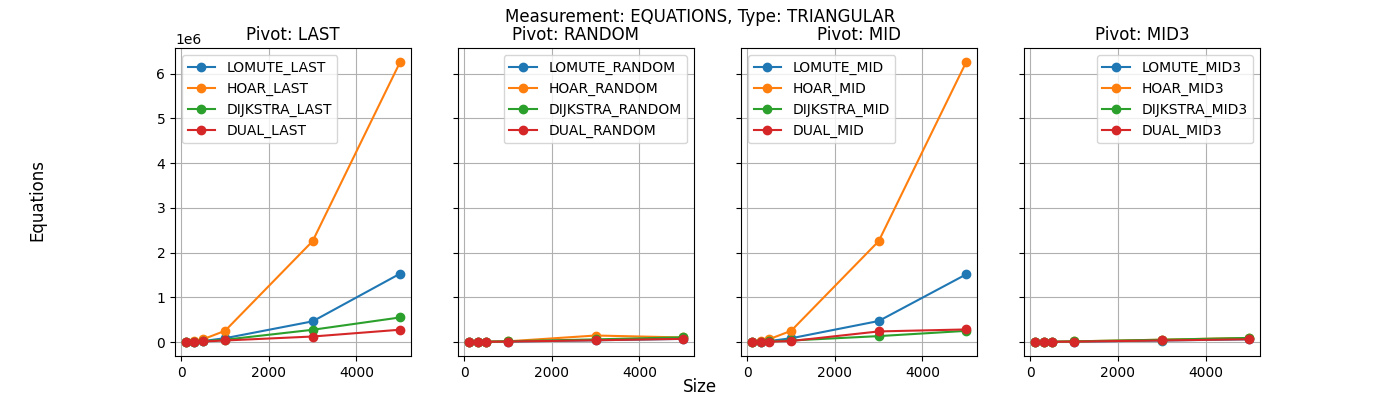
\includegraphics[scale=0.5]{triangular_Equations_6_numbers.png}
        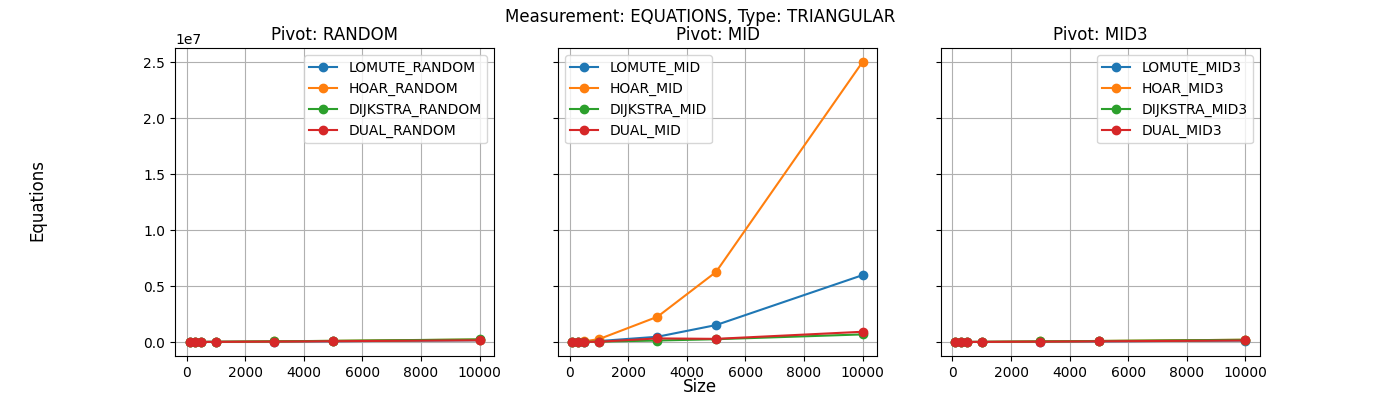
\includegraphics[scale=0.5]{triangular_Equations_3_pivots_7_numbers.png}
        \newline
    \textbf{Операцiй обмінів:}
    \newline
        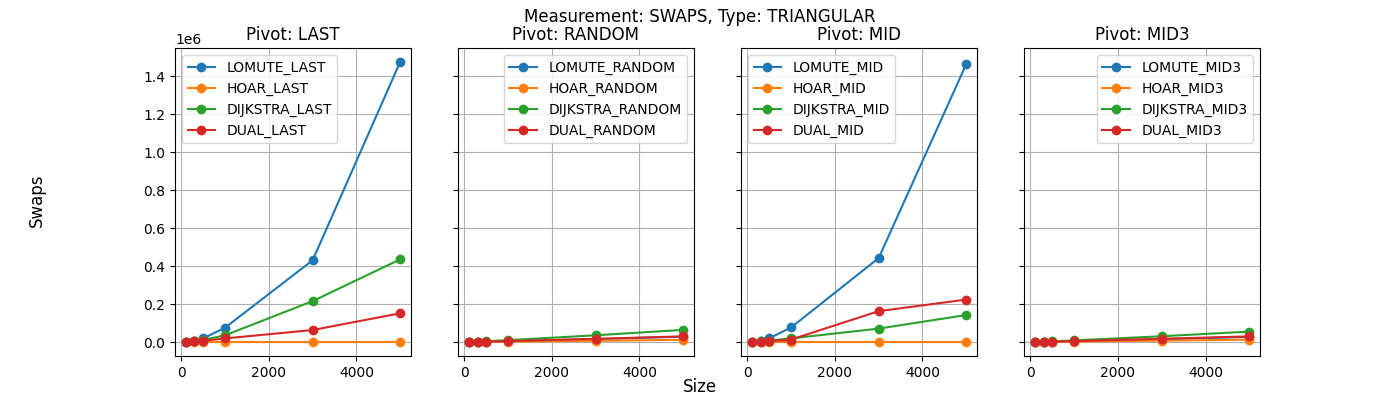
\includegraphics[scale=0.5]{triangular_Swaps_6_numbers.png}
        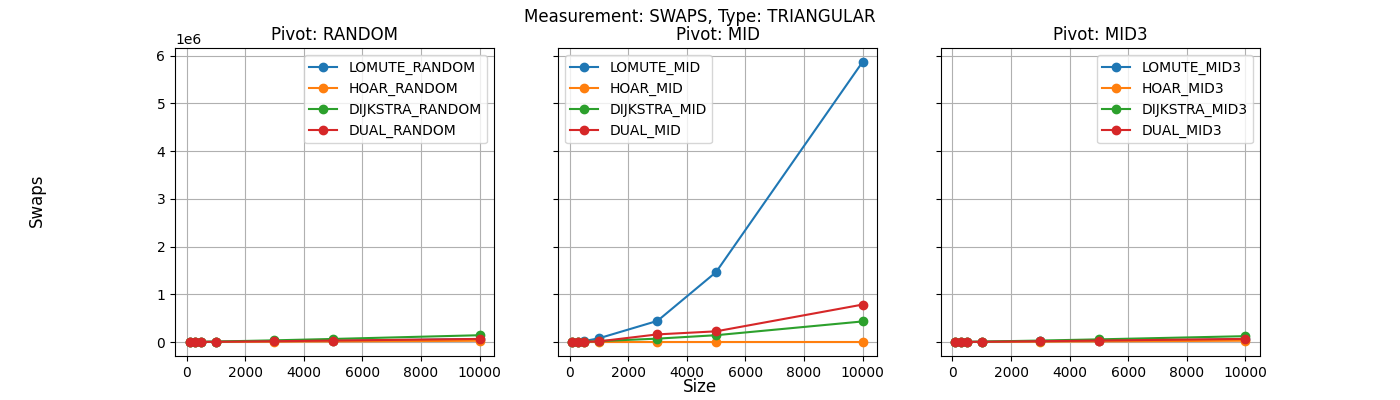
\includegraphics[scale=0.5]{triangular_Swaps_3_pivots_7_numbers.png}
        \newline
    \newpage
    \textbf{Використано пам’ятi:}
    \newline
        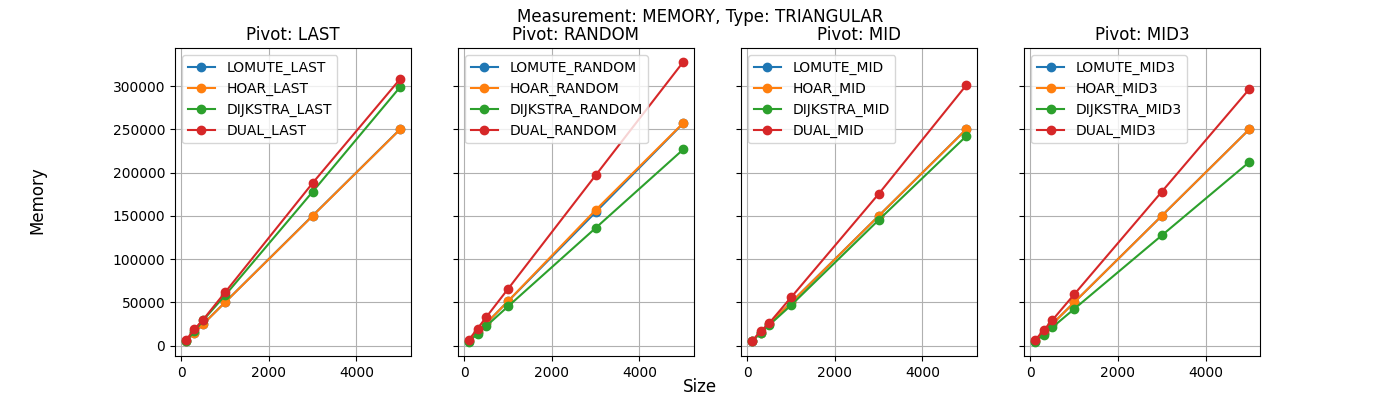
\includegraphics[scale=0.5]{triangular_Memory_6_numbers.png}
        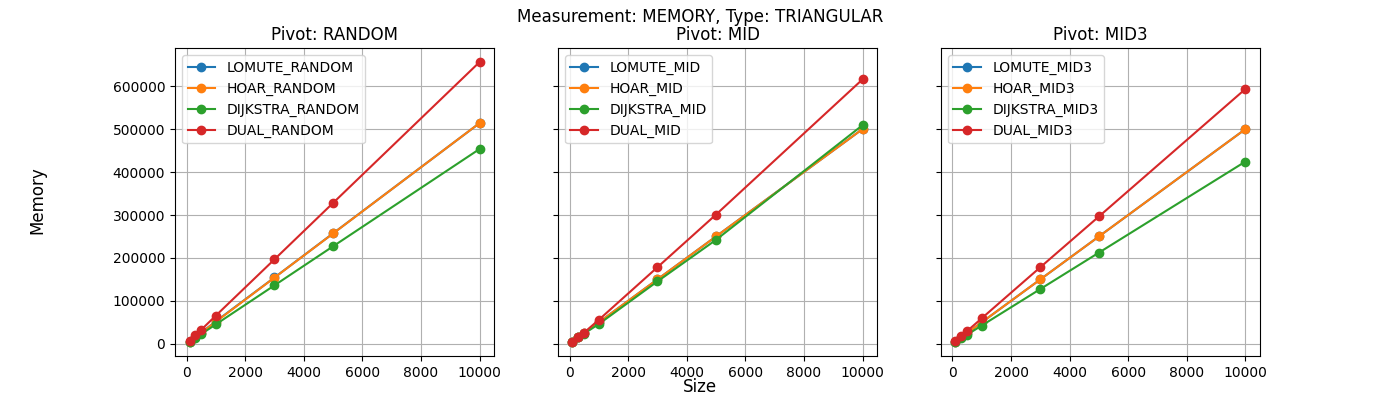
\includegraphics[scale=0.5]{triangular_Memory_3_pivots_7_numbers.png}
    \subsection{Висновки для "трикутних" масивів:}
    \begin{enumerate}
        \item 
    \end{enumerate}
    \newpage

\end{document}